\documentclass{beamer}
\usepackage{amsmath}
\usepackage{beamerthemesplit}
\usepackage{graphicx} % Required to insert images
\usepackage[utf8]{inputenc}
\usepackage{tcolorbox}
\usepackage[T1]{fontenc}
\usepackage{lmodern}
\usepackage{verbatim}
\usepackage{listings}

\title{Dominion Datamining}
\author[TAGNAOUTI, LOPEZ, VER VALEM, BAYOL]{Khaoula TAGNAOUTI, Liliana LOPEZ, Willian VER VALEM, Elmer BAYOL}

\begin{document}
\maketitle

\begin{frame}
  \frametitle{Introduction}
  \framesubtitle{Le contexte du projet}
  
  \begin{itemize}
  \item Un serveur ouvert d'Octobre 2010 à Mars 2013
    \item 12 Millions de logs à traiter (dont la taille générale est 13Go)
    \item Un Wiki offre des conseils au niveau de la stratégie
  
  \end{itemize}
\end{frame}
  
  \begin{frame}
  \frametitle{Introduction}
  \framesubtitle{Le but du projet}
  Dominion DataMining est un programme qui se compose de trois parties principales:
  \begin{itemize}
  \item Modélisation des donées
  \item Stockage des données
  \item Analyse des données
  \end{itemize}
\end{frame}

\begin{frame}
  \frametitle{Introduction}
  \framesubtitle{Classe de l'utilisateur et caractéristiques}
 
  \begin{itemize}
    \item Acteurs physiques:
     ~~\\
     \textit{Utilisateur}
      ~~\\
    \item Acteurs de système:  
      ~~\\
     \textit{Parser}
       ~~\\
     \textit{Analyseur}
      ~~\\
     \textit{Base de données}
      ~~\\
     
  \end{itemize}

\end{frame}
  

\begin{frame}
  \frametitle{Fonctionnalités}
  \begin{itemize}
  \item Parser
  \item Stockage des données
  \item Calcul d'elo
  \end{itemize}
\end{frame}

\begin{frame}
  \frametitle{Fonctionnalités}
  \framesubtitle{Parser}
  \begin{itemize}
  \item 99.8\% des logs sont parsés
  \item Seul le header est parsé
  \item Est capable de travailler avec les logs compressés
  \end{itemize}
\end{frame}

\begin{frame}
  \frametitle{Fonctionnalités}
  \framesubtitle{Stockage des données}
  \begin{itemize}
  \item Stockage des parties
  \item Stockage d'elo global pour chaque joueur
  \item Stockage de liste des parties d'un joueur
  \end{itemize}
\end{frame}

\begin{frame}
  \frametitle{Fonctionnalités}
  \framesubtitle{Stockage des données}
  Exemple de structure stockée dans la base de données:\newline
  \begin{center}
    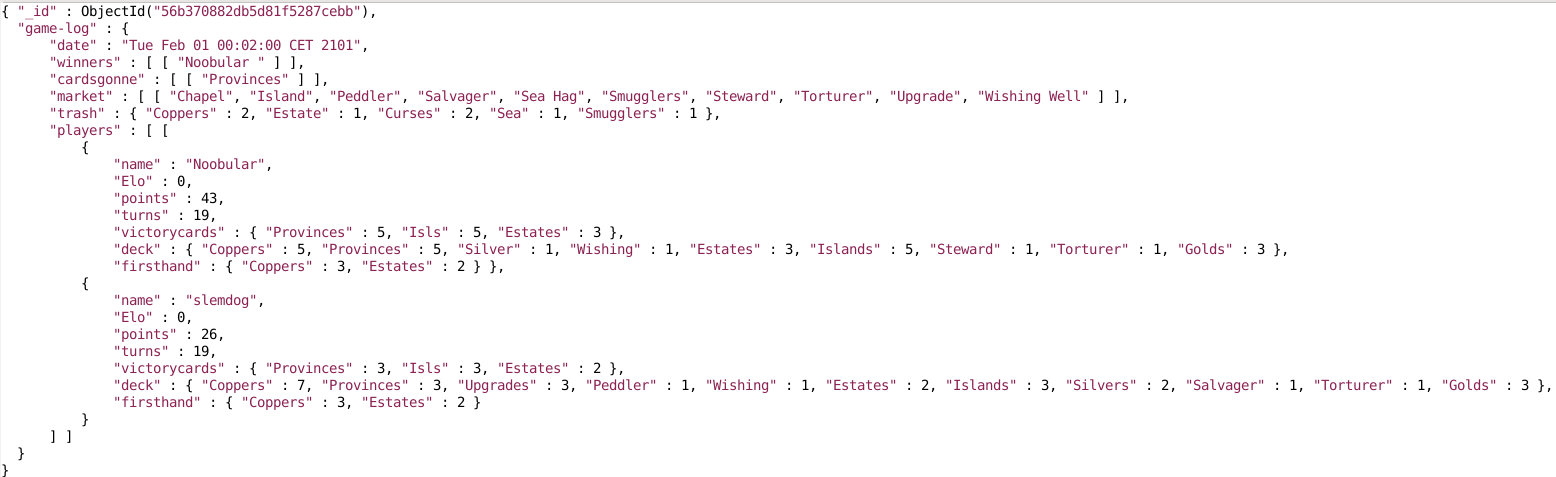
\includegraphics[scale=0.21,keepaspectratio]{code}
  \end{center}
\end{frame}

\begin{frame}
  \frametitle{Fonctionnalités}
  \framesubtitle{Calcul d'elo}
  \begin{itemize}
  \item Chaque partie est prise en ordre chronologique
  \item Prise en compte de l'elo global
  \item Mise a jour du nouvel elo global du joueur
  \item Ajout de l'elo du joueur au moment de la partie (ne varie pas)
  \end{itemize}
\end{frame}

\begin{frame}
  \frametitle{Fonctionnalités}
  \framesubtitle{Calcul d'elo}
  \begin{center}
    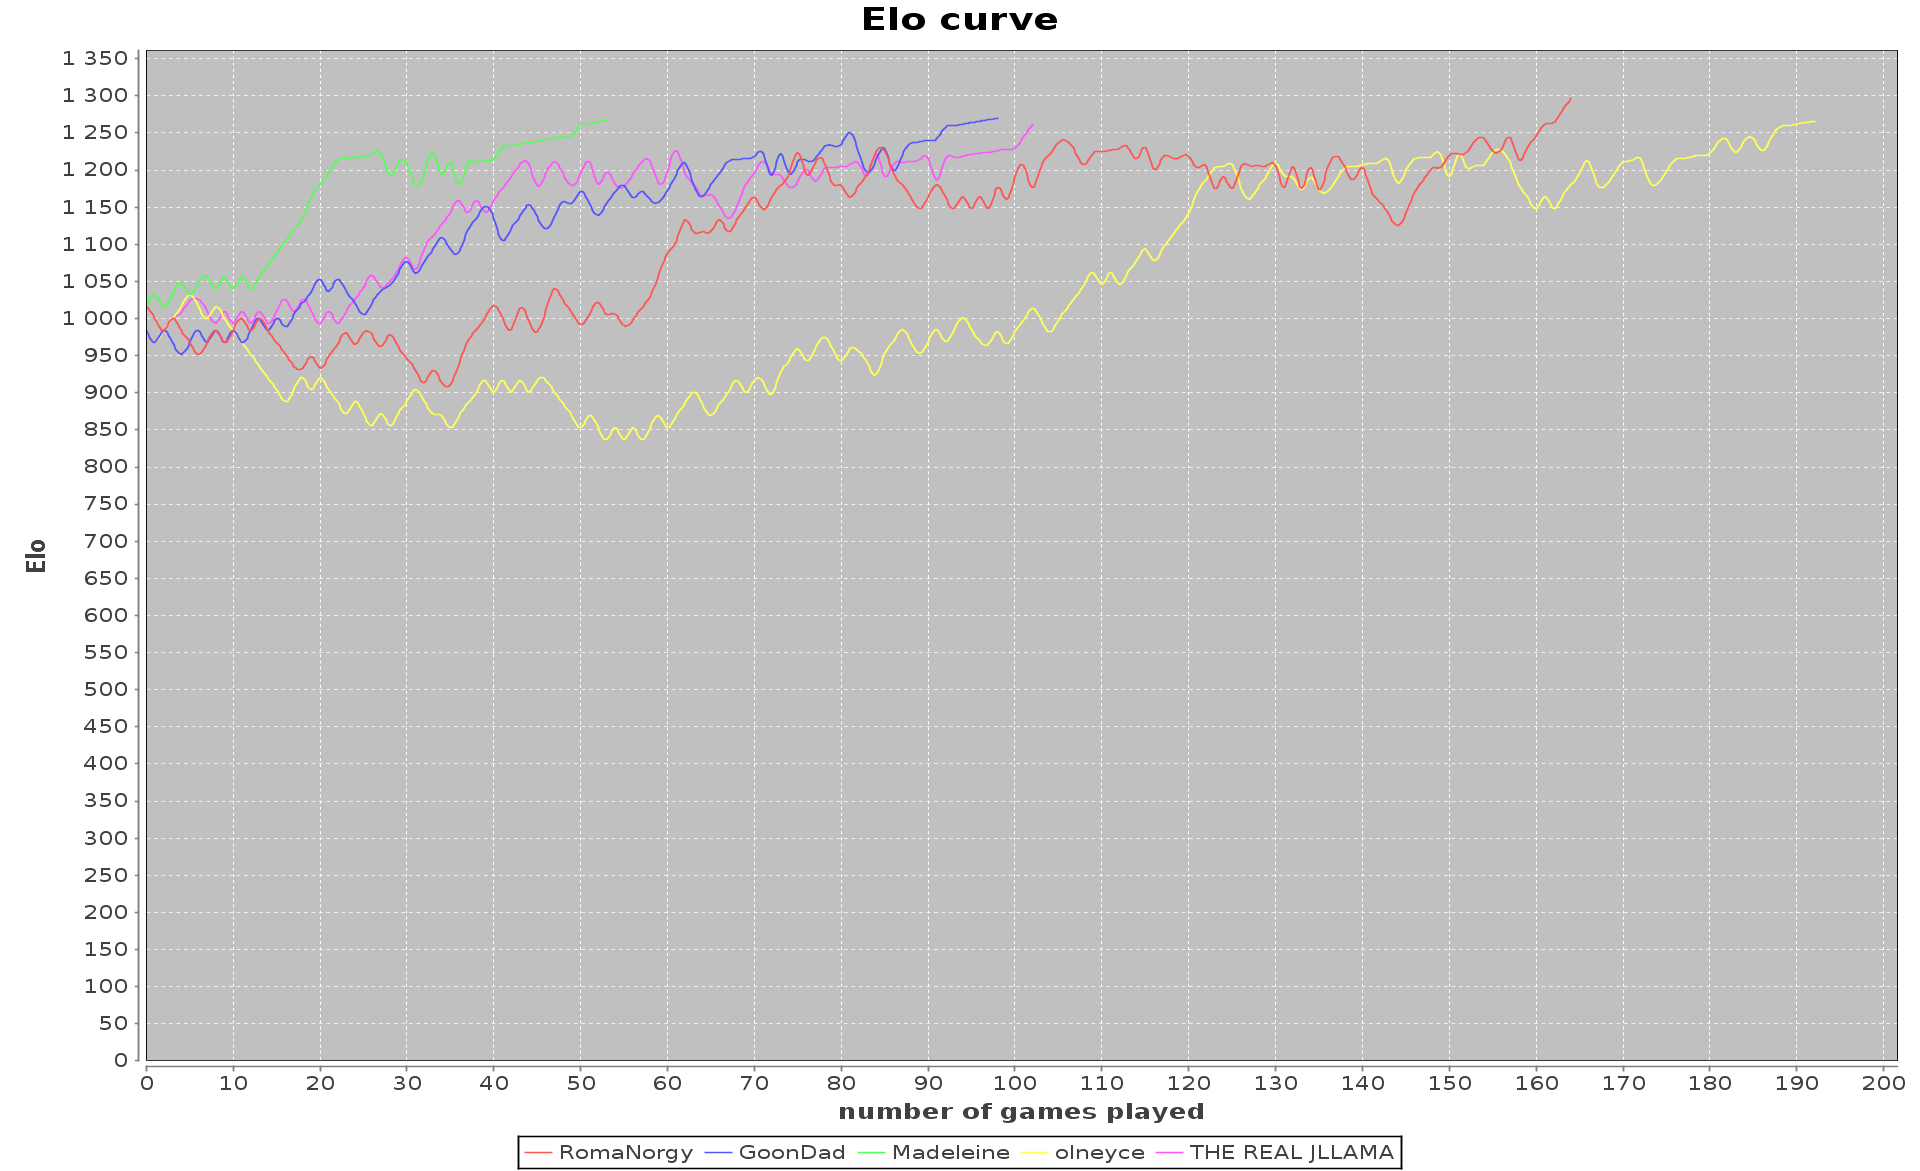
\includegraphics[scale=0.15,keepaspectratio]{elo}
  \end{center}
\end{frame}

\begin{frame}
  \frametitle{Architecture}
  \begin{center}
    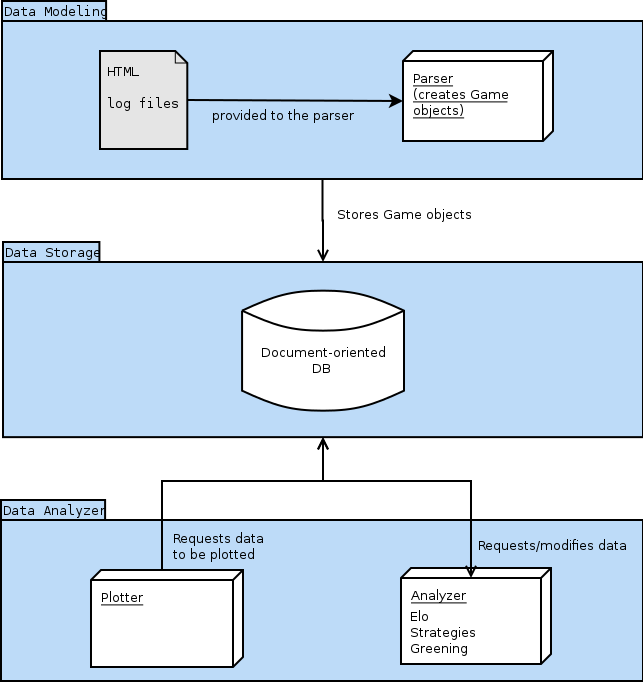
\includegraphics[scale=0.30,keepaspectratio]{globalArch_v2}
    \end{center}
\end{frame}

\begin{frame}
  \frametitle{Architecture}
  \begin{center}
    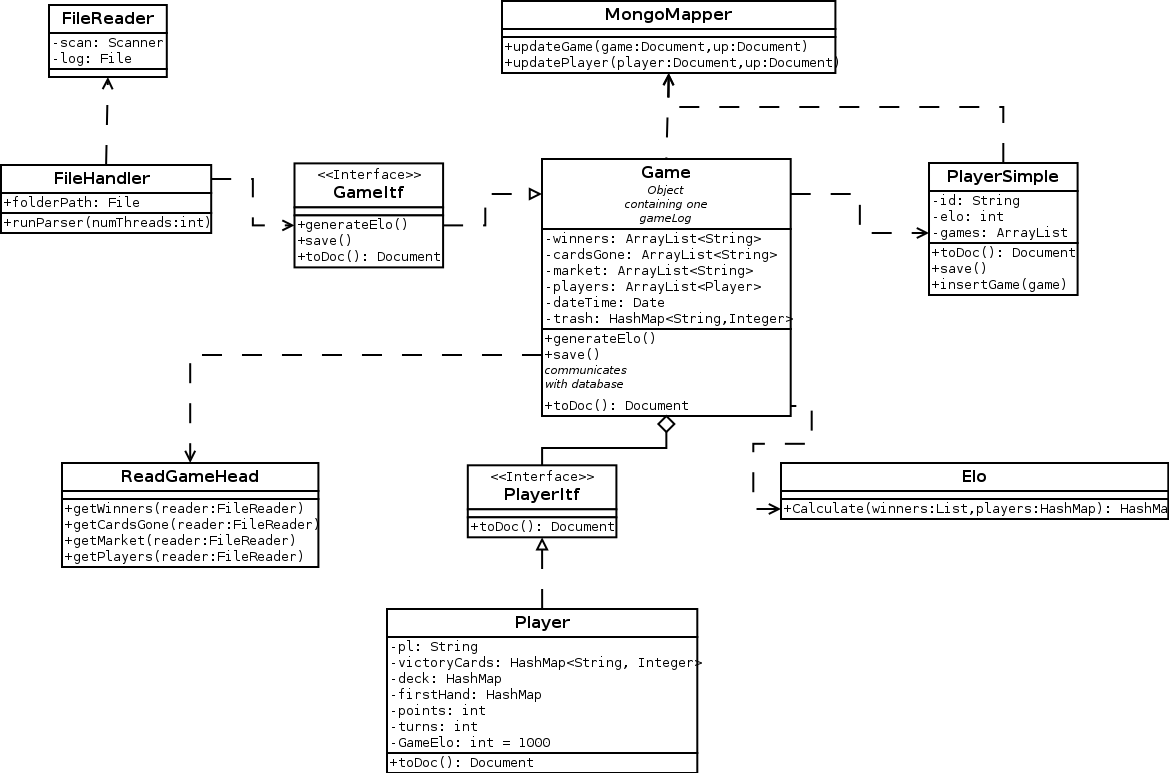
\includegraphics[scale=0.27,keepaspectratio]{parserArch}
    \end{center}
\end{frame}

\begin{frame}
  \frametitle{Aspects techniques}

  \begin{itemize}
  \item Choix techniques
  \item Algorithmes
  \item Bugs et problèmes
  \end{itemize}
\end{frame}

% \begin{tcolorbox}[colback=green!5,colframe=green!40!black,title=A nice heading]
% \end{tcolorbox}

\begin{frame}
  \frametitle{Choix techniques}
\begin{tcolorbox}[colback=green!5,colframe=green!40!black,title=Choix d'implémentation]
  \begin{center}
    
\includegraphics[scale=0.30,keepaspectratio]{maven}\\
    
\includegraphics[scale=0.30,keepaspectratio]{mongojava}
    \end{center}
\end{tcolorbox}
\end{frame}


\begin{frame}
  \frametitle{Algorithmes}
\begin{tcolorbox}[colback=green!5,colframe=green!40!black,title=Parser]
  \begin{itemize}
  \item un mélange jsoup + split
  \item et beaucoup de recherches regex
  \end{itemize}
\end{tcolorbox}
\begin{tcolorbox}[colback=green!5,colframe=green!40!black,title=Elo]
  \[
    {R_{x}} = {R_{x}} + 32 * (v - \frac{10^{{R_{x}}/400}}{\sum_{n=0}^{np} Rn})
  \]
v = 1 si le joueur gagne et 0 si il perd
\end{tcolorbox}
\end{frame}


\begin{frame}
  \frametitle{Bugs et Problèmes}
\begin{tcolorbox}[colback=green!5,colframe=green!40!black,title=Noms d'utilisateur]
  \begin{itemize}
    \item  cats and dogs living together
    \item  gime all yo points
      \item hi, gl, hf, yada, yada, yada.
       \item (>\textasciicircum o \textasciicircum)> <(*o*)> <(\textasciicircum
         o \textasciicircum<)
  \end{itemize}

\end{tcolorbox}

\begin{tcolorbox}[colback=green!5,colframe=green!40!black,title=Performance]
  \begin{itemize}
  \item fichiers compressés
  \item grosse utilisation du disque
  \end{itemize}
\end{tcolorbox}
\end{frame}

\begin{frame}
  \frametitle{Questions}
  \begin{center}
    
\includegraphics[scale=0.21,keepaspectratio]{qa}
  \end{center}
\end{frame}

\end{document}
